
\section{Introduction}

In the end of section ~\ref{chp:SOLO_Quite_time}, \citet{Mason-2021-SolOQuietTime} reports the radial gradient of \ac{ACR} oxygen and helium-4 with energy of 4.4 MeV/nuc inside 1 au. The results are based on the measurement in 2020 and the intensities of particle are plotted as a function of three radial gradients. Though the relative larger uncertainty which is due to the limited count number, the results suggest a consistent oxygen gradient with the observation from Helios and \ac{PSP} \citep{Rankin2021ApJ,Marquardt2018AA}.

As of 2023, \ac{SolO} has finished its fifth orbit and continues its trip in the inner heliosphere, providing more valuable measurements by \ac{EPD} for the study of \ac{ACR} radial gradient of \ac{ACR}. 
In this chapter, we will employ the new data from \ac{HET} onboard \ac{SolO} and present the first observation of the \ac{ACR} heliums in the inner heliosphere between 2020 and 2022. Possible interuptions including \acp{SEP}, periodically appeared compression regions and the long term solar modulation are properly considered. Moreover, the helium flux measured by \ac{EPHIN} onboard \ac{SOHO} is utilized to derive the ratio of \ac{SolO} and \ac{SOHO}/\ac{EPHIN} in order to remove the effect of solar modulation. Our preliminary results show the consistene helium flux level between \ac{SolO} and \ac{SOHO}/\ac{EPHIN} and the radial gradient of helium-4 is consistent with the previous results from \ac{PSP} within the uncertainty.

Below we report the details of the data analysis and summary of the results, although some results are still in the preliminary phase. We will continue the data analysis in the future and the final version of the paper is in preparation for publication.



\section{Background}
I list the center sentence here and you will fill and expand them later

The Anomolous cosmic ray are the energetic particles that widely existed in the heliosphere with energy of tens of MeV/nuc.


source of ACR is believe to be located around the temination shock,  [What is the evidence, find the citation]

ACR dominate the few tens of MeV/nuc energy range.

Including what particles,

When traveling inward, several factors affect the transport of the particle in the heliosphere: (a) diffusion, (b) adabitice expanding,  (c) drift  [expand and find the right citation]

The drift direction of energetic particle are different during opposite solar polarity. A> 0, what ? A<0 what? 


The spatial distribution is a perfect test of the transport theory of the cosmic ray particles in the heliesphere.
\todo[inline]{More here about the spatial and its meaning to the our study}
Below are two type of equation that we could use to calculate the radial gradient of charged particles.



Specially, The radial gradient is one of the key parameters to constrain particle transport. The radial gradient could be express as \cite{Rankin2021ApJ...912..139R} :
\begin{equation}
    g_r = \frac{1}{f}\frac{\partial{f}}{\partial{r}} = \frac{\partial{\mathrm{ln} f}}{\partial{r}}
\end{equation}

Where $g_r$ represents the radial gradient component under the assumption that the latitude gradient are neglectable. $f$ is the differential flux and $r$ is the radial distance. The radial gradient could be easily derived by fitting it to a linear equation according to the least minimum square method.

Previously, the observation of the radial gradient of ACR helium (10- 50 MeV/nuc) are mainly carried on by the Voyager and Helium for the region outside of the 1 AU, except PSP, which carried on the most updated observation of the radial gradient below 1AU.


Another interesting measurements are the time variation of the radial and latittude gradient between consecutive solar cycle, as predicted from the cosmic-ray transportation model.[Add more]  In this study, together with the previous literature result and the new measurement from PSP and SOLO, we try to give the temporal variation of the radial gradient of ACR helium between different solar minimum and preliminary result of the gradient chagne from solar minimum to the solar maximum.


Solar orbiter EPD is the energetic particle suite used for the detection of high energy particles. The energy coverage of EPD including the energy range of solar energetic particles, Anomalous cosmic rays, and the high energy particle that dominated by the galactic cosmic ray during the solar quiet time.

SOLO is the new satellite launched at the solar minimum 24/25 and moves ecliptic close to the sun. 
The High energetic parßticle telescope onboard the SOLO makes the measurement of the radial gradient less than 1 au possible.
After several venus flyby and earth flyby SOLO could reach 0.3 au
The orbit of the solo in which helioscentriccoordinate.

In this report, we organized the content as following: We first introduce the data and instrument we used in this work, which including the SOLO/HET, SOHO/EPHIN, STEREO/LET and possiblely LND. In chapter 3 we give the overview of the observation of the helium-4 between 2020 and 2022 when in the second half, SEPs frequently happens and the overall cross-calibration between different instrument

In section4, we explain the several kind of effect that could disturbe the constanct background and show how the result are affected by different method.  In the end, we conclude.


\begin{figure}
    \centering
    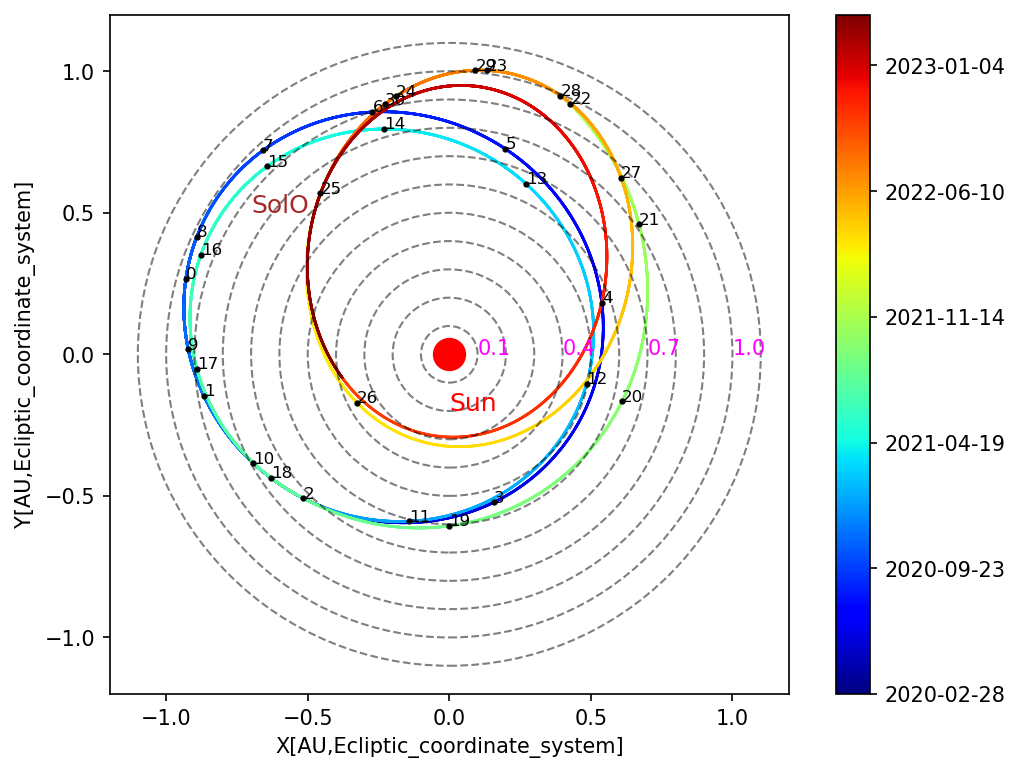
\includegraphics[width=0.8\textwidth]{images/ACR/SOLO_orbit_helioscentric_carrington_orbitnumber.png}
    \caption{The orbit of the SOLO.}
    \label{fig:SOLO_orbit}
\end{figure}

\begin{figure}
    \centering
    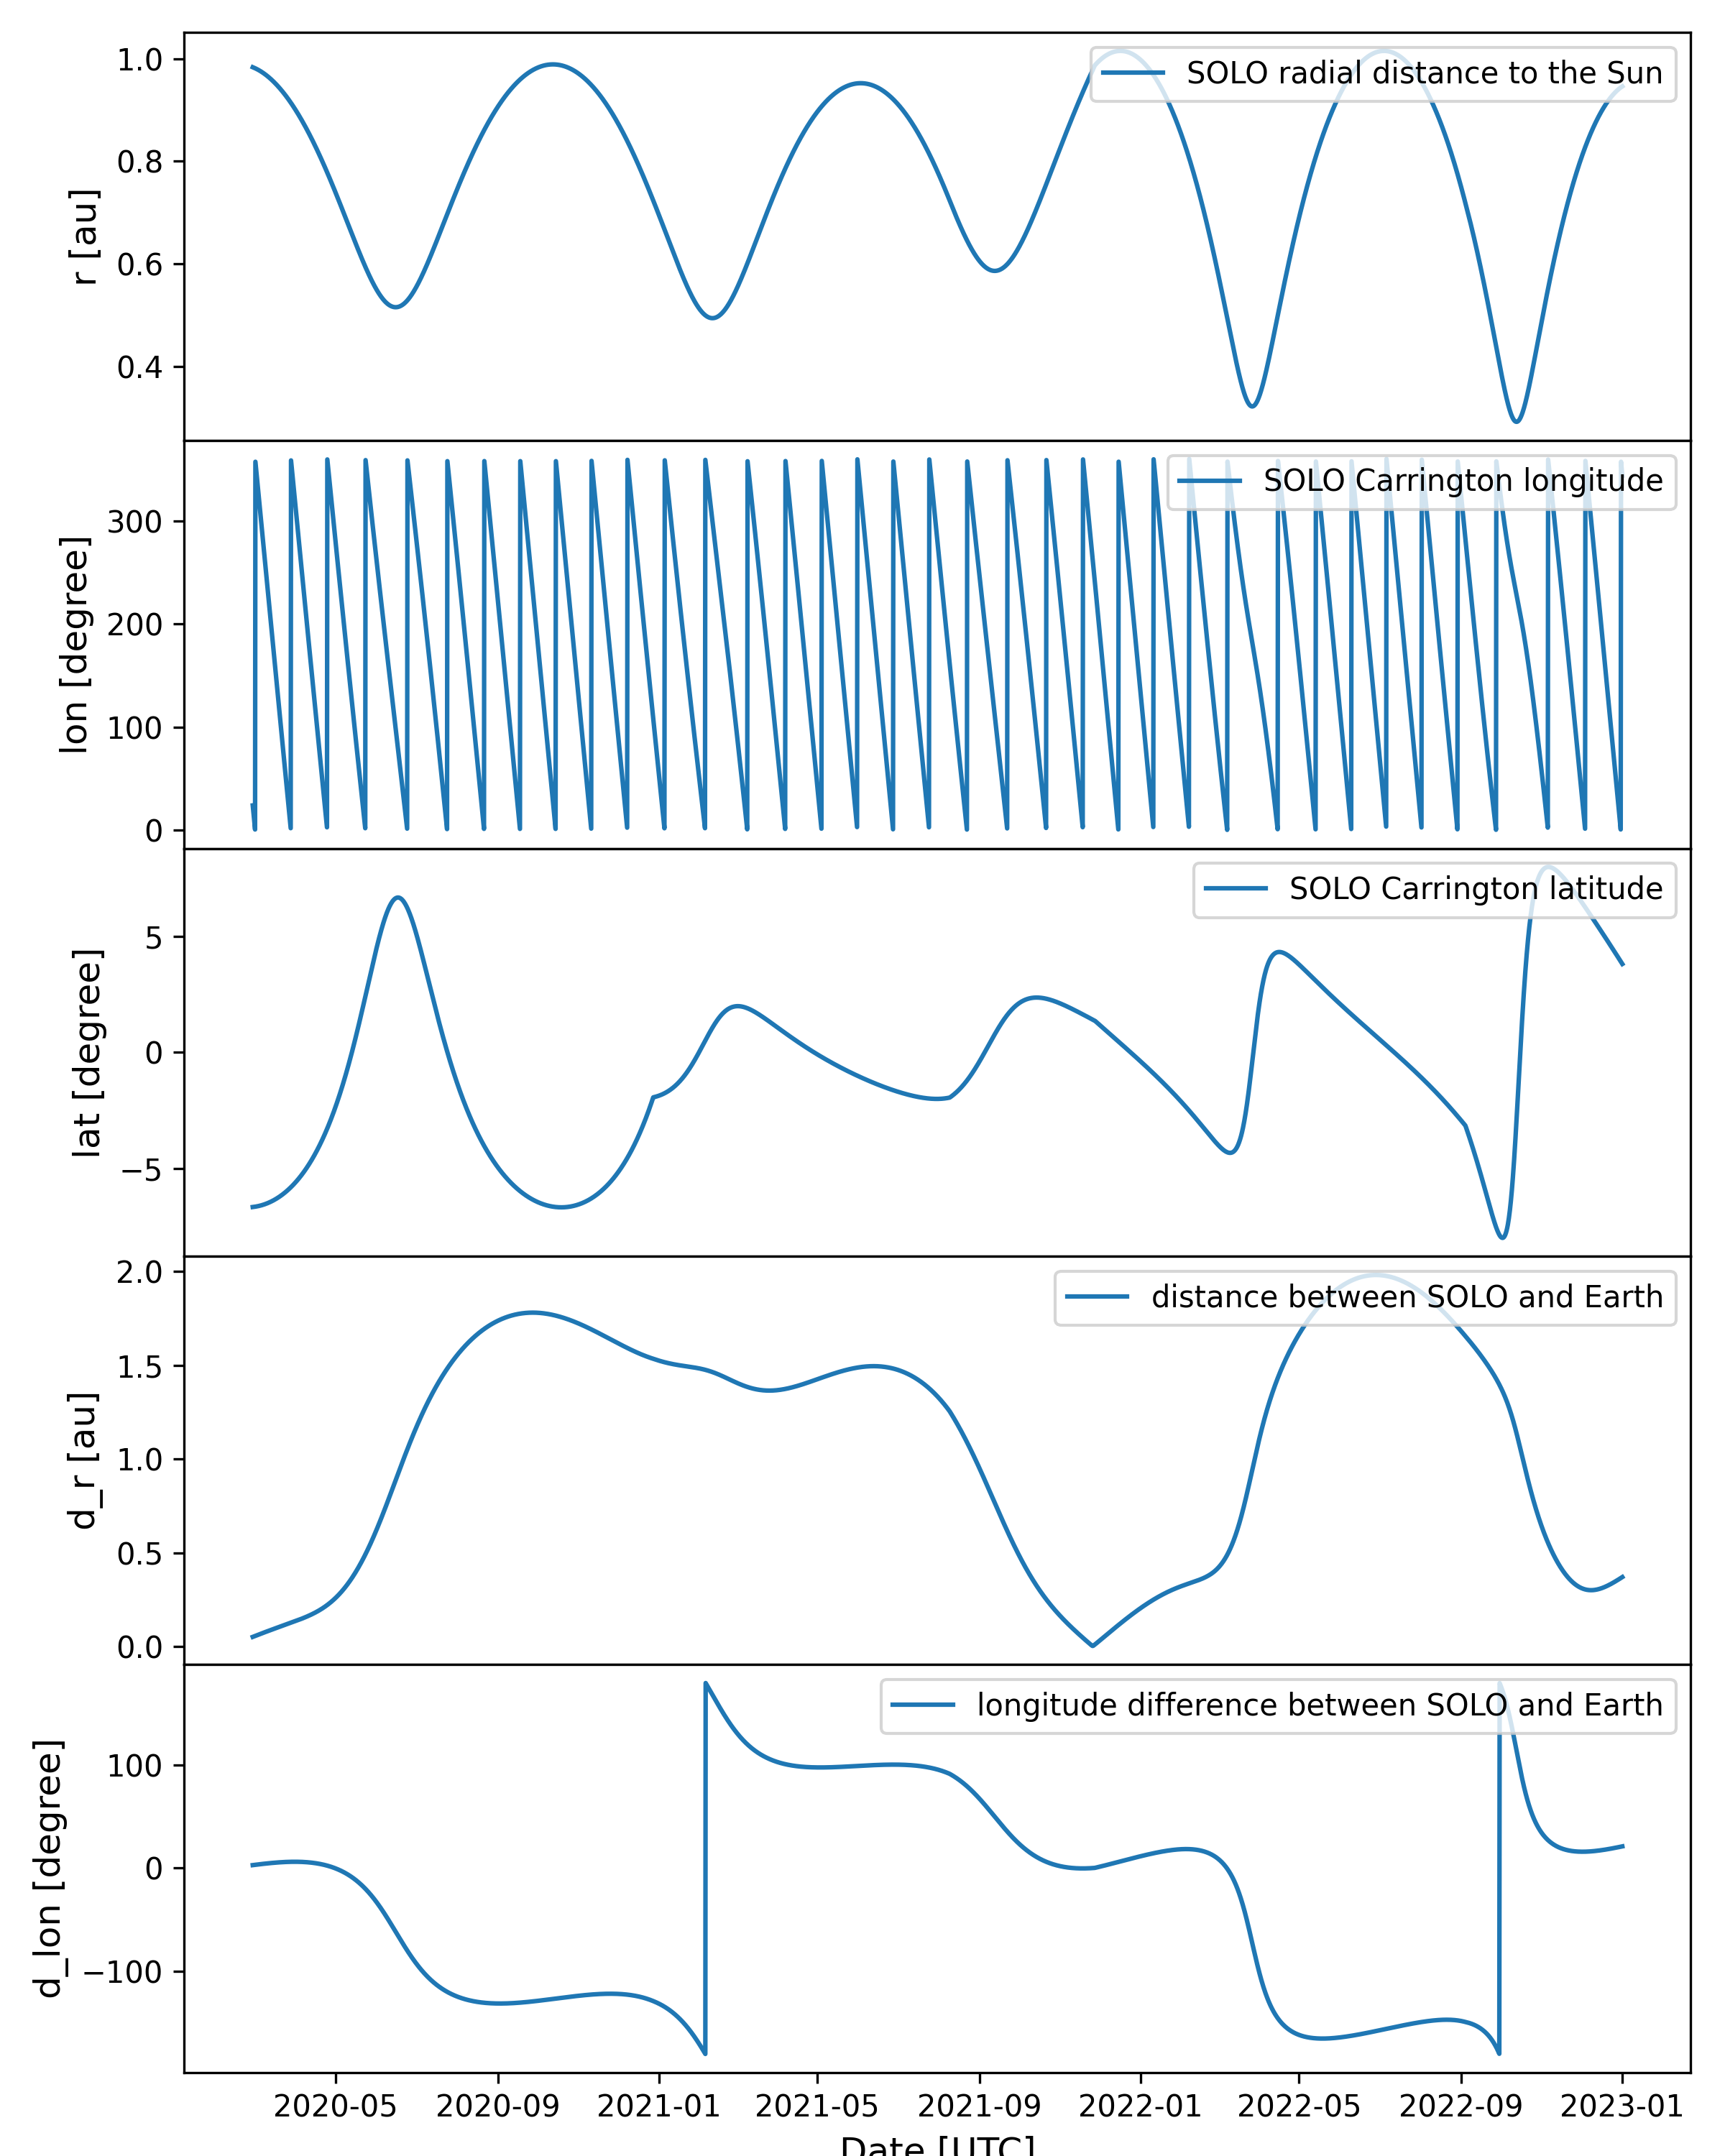
\includegraphics[width = 0.7\textwidth]{images/ACR/SOLO_orbit_helioscentric_2.png}
    \caption{The radial distance (top), carrignton longitude (second from top), latitude, distance and delta longitude between SOLO and SOHO ( bottom two)}
    \label{fig:SOLO_orbit_2}
\end{figure}


\section{Instrument}

\begin{figure}
    \centering
    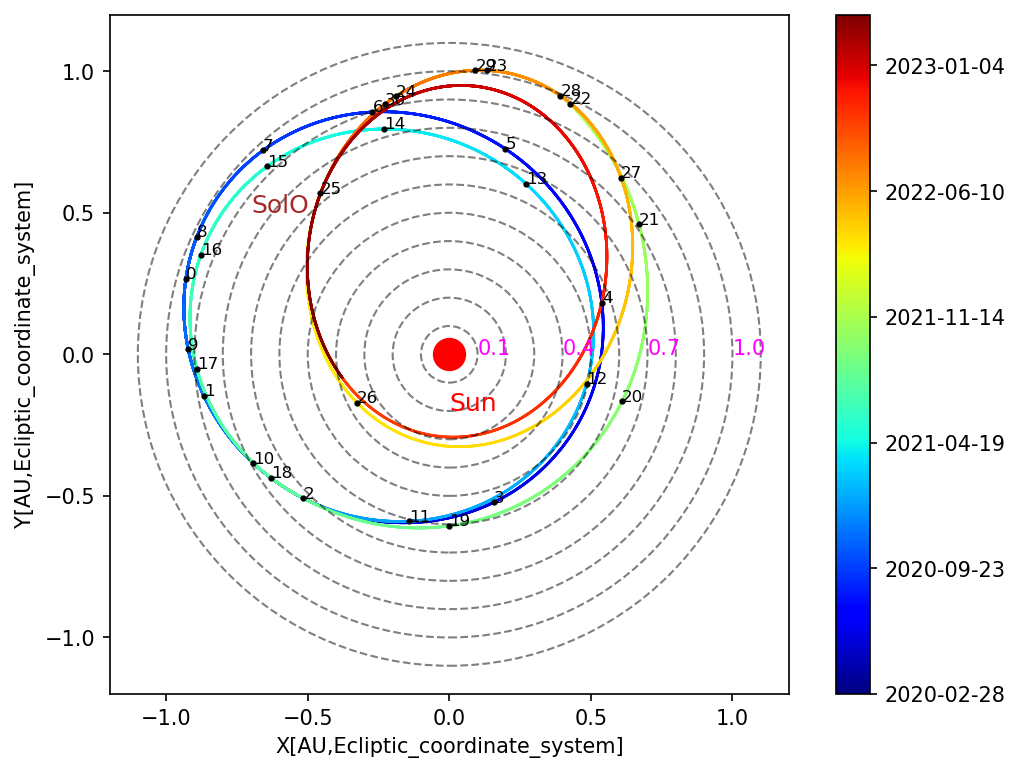
\includegraphics[width=0.8\textwidth]{images/ACR/SOLO_orbit_helioscentric_carrington_orbitnumber.png}
    \caption{The orbit of the SOLO.}
    \label{fig:SOLO_orbit}
\end{figure}

\begin{figure}
    \centering
    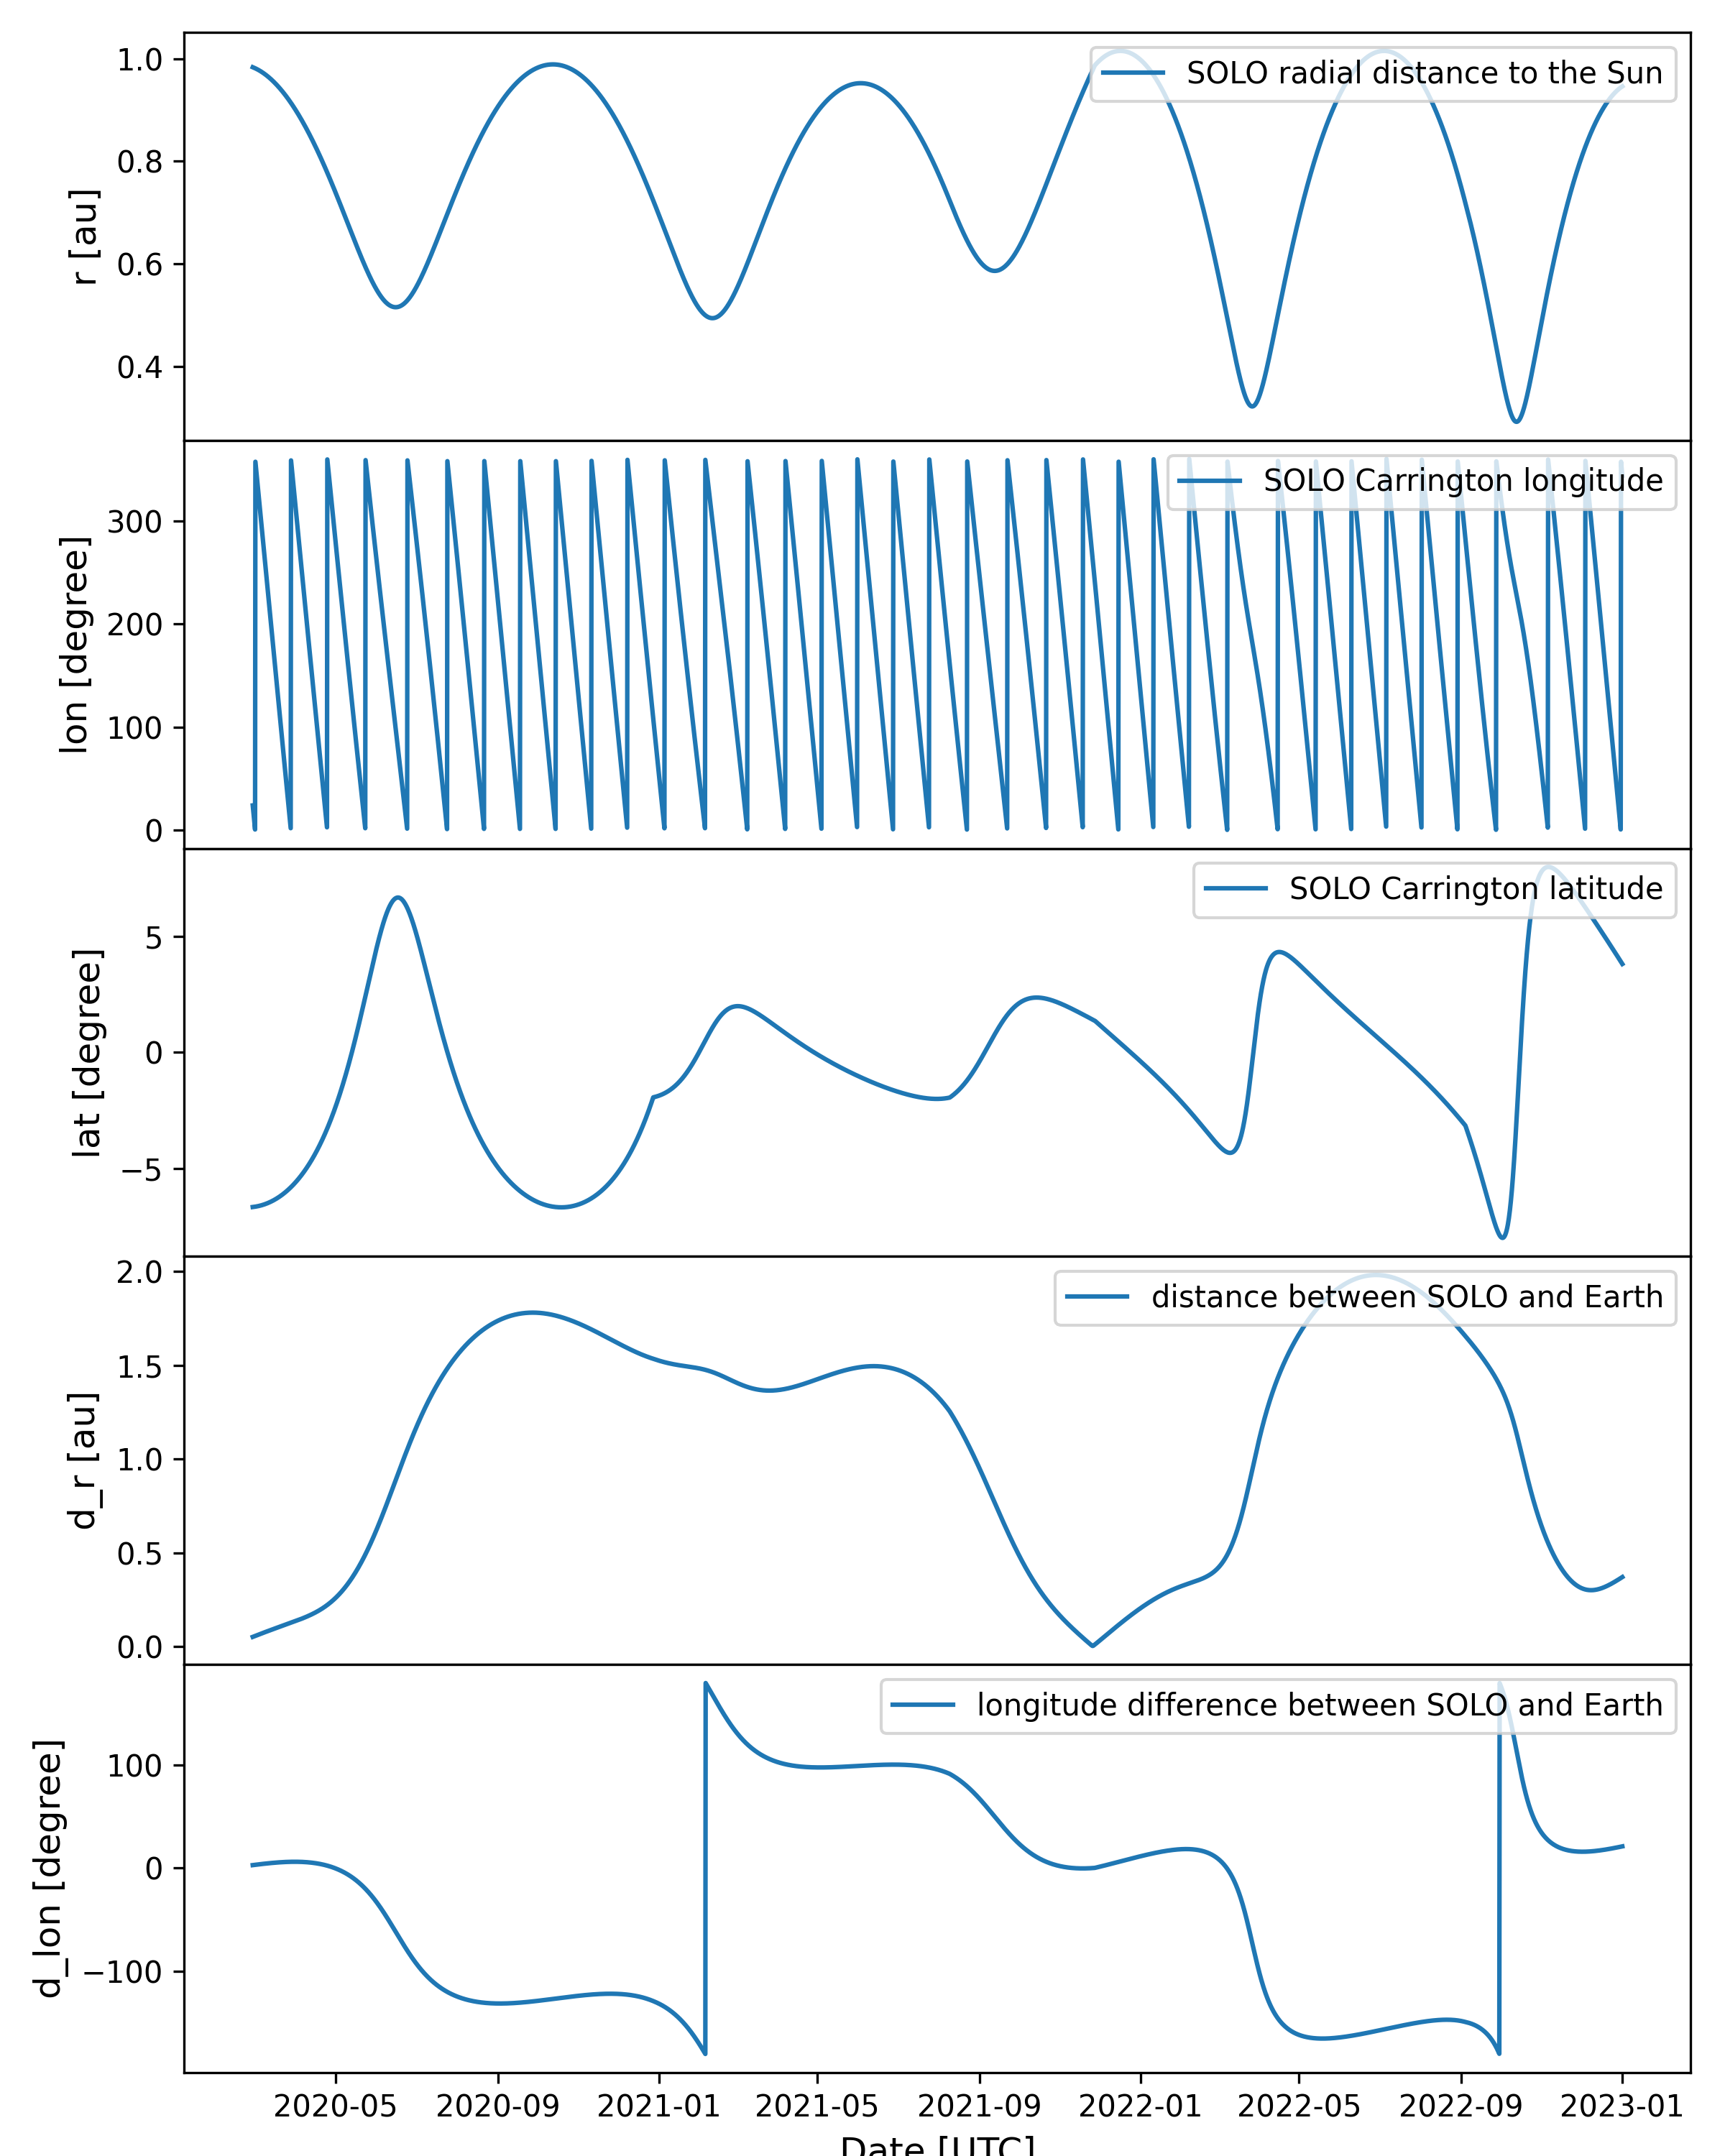
\includegraphics[width = 0.7\textwidth]{images/ACR/SOLO_orbit_helioscentric_2.png}
    \caption{The radial distance (top), carrignton longitude (second from top), latitude, distance and delta longitude between SOLO and SOHO ( bottom two)}
    \label{fig:SOLO_orbit_2}
\end{figure}

We use HET,
We recombined data products
We summed up data products from four different directions

We use SOHO/EPHIN

We ACE/SIS
We use STA/LET
We use LND
The latter three are just used as an direct comparison and  we do not use them to derive the radial gradient.

\section{Observation and data analysis}

\subsection{Overview observation between 2020 and 2022 and the cross calibration between four instruments}


We first present the overview observation of \ac{SolO}/\ac{HET} of heavier ions, including helium, carbon, nitrogen and oxygen


\begin{figure}
    \centering
    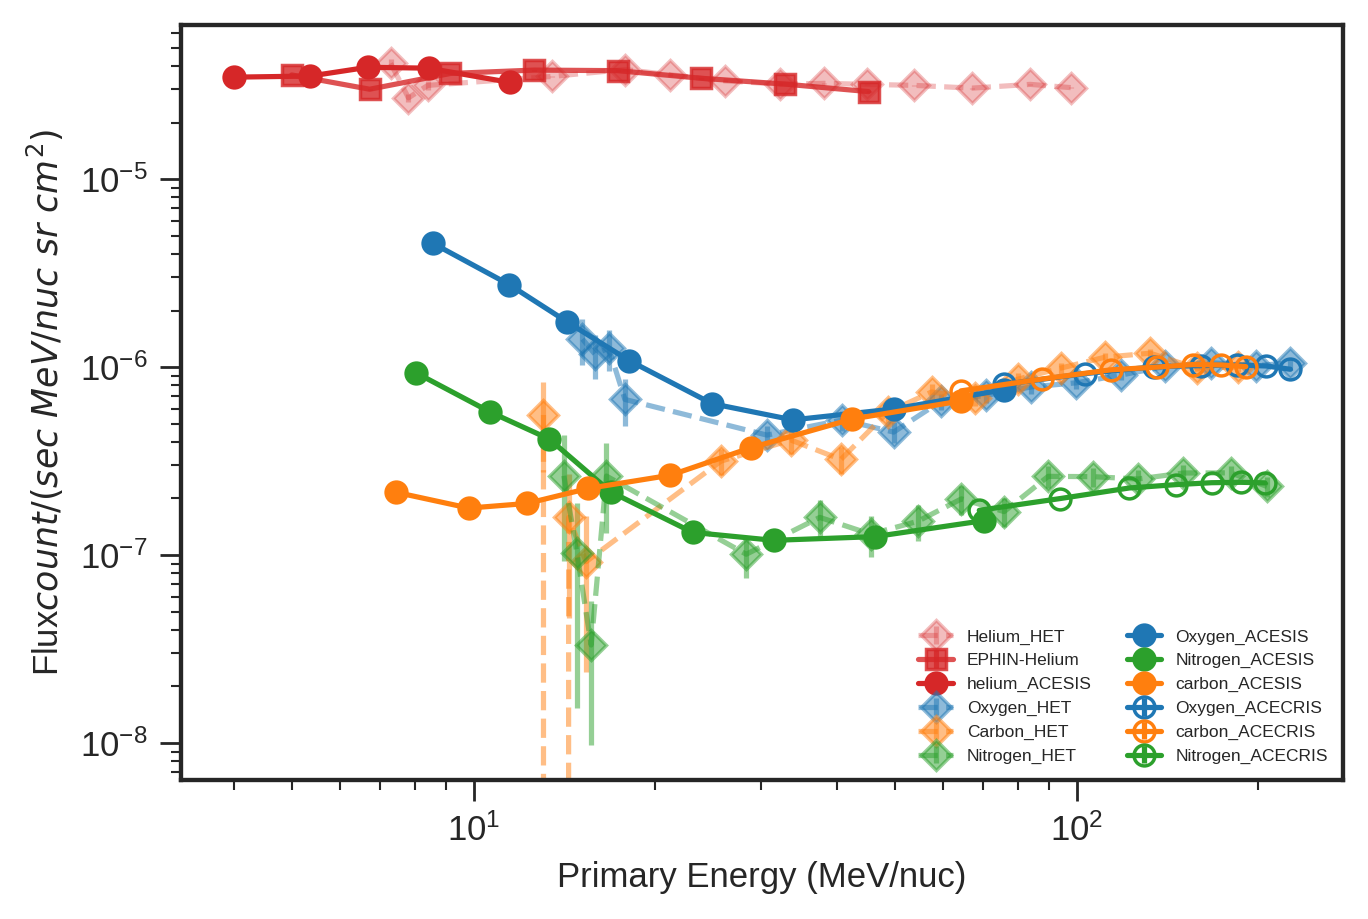
\includegraphics[width = 0.8\textwidth]{images/ACR/Overviewspectra_twoyear_wto_SEP.png}
    \caption{The helium-4 (red), carbon (orange), nitrogen (green) and oxygen (blue) spectrum averaged between 2020 and 2022. The \ac{SEP} events are removed from the data. The measurements are from \ac{SolO}/\ac{HET}, \ac{SOHO}/\ac{EPHIN} and \ac{ACE}. \TODO{maybe add the penetrating helium?}}
    \label{fig:overview}
\end{figure}

The direct comparison between the heavy ion spectra show the general agreement between the \ac{SolO} and the instrument in L1 points, suggesting the good instrument performance of \ac{SolO}/\ac{HET}.


The temperol variation of the Helium measurement from different instrument including HET, EPHIN, LET and LND.
The solar minimum is still continuing between 2020 and 2021 when GCR quite, SEP rare.

After SEP increase
\begin{figure}
    \centering
    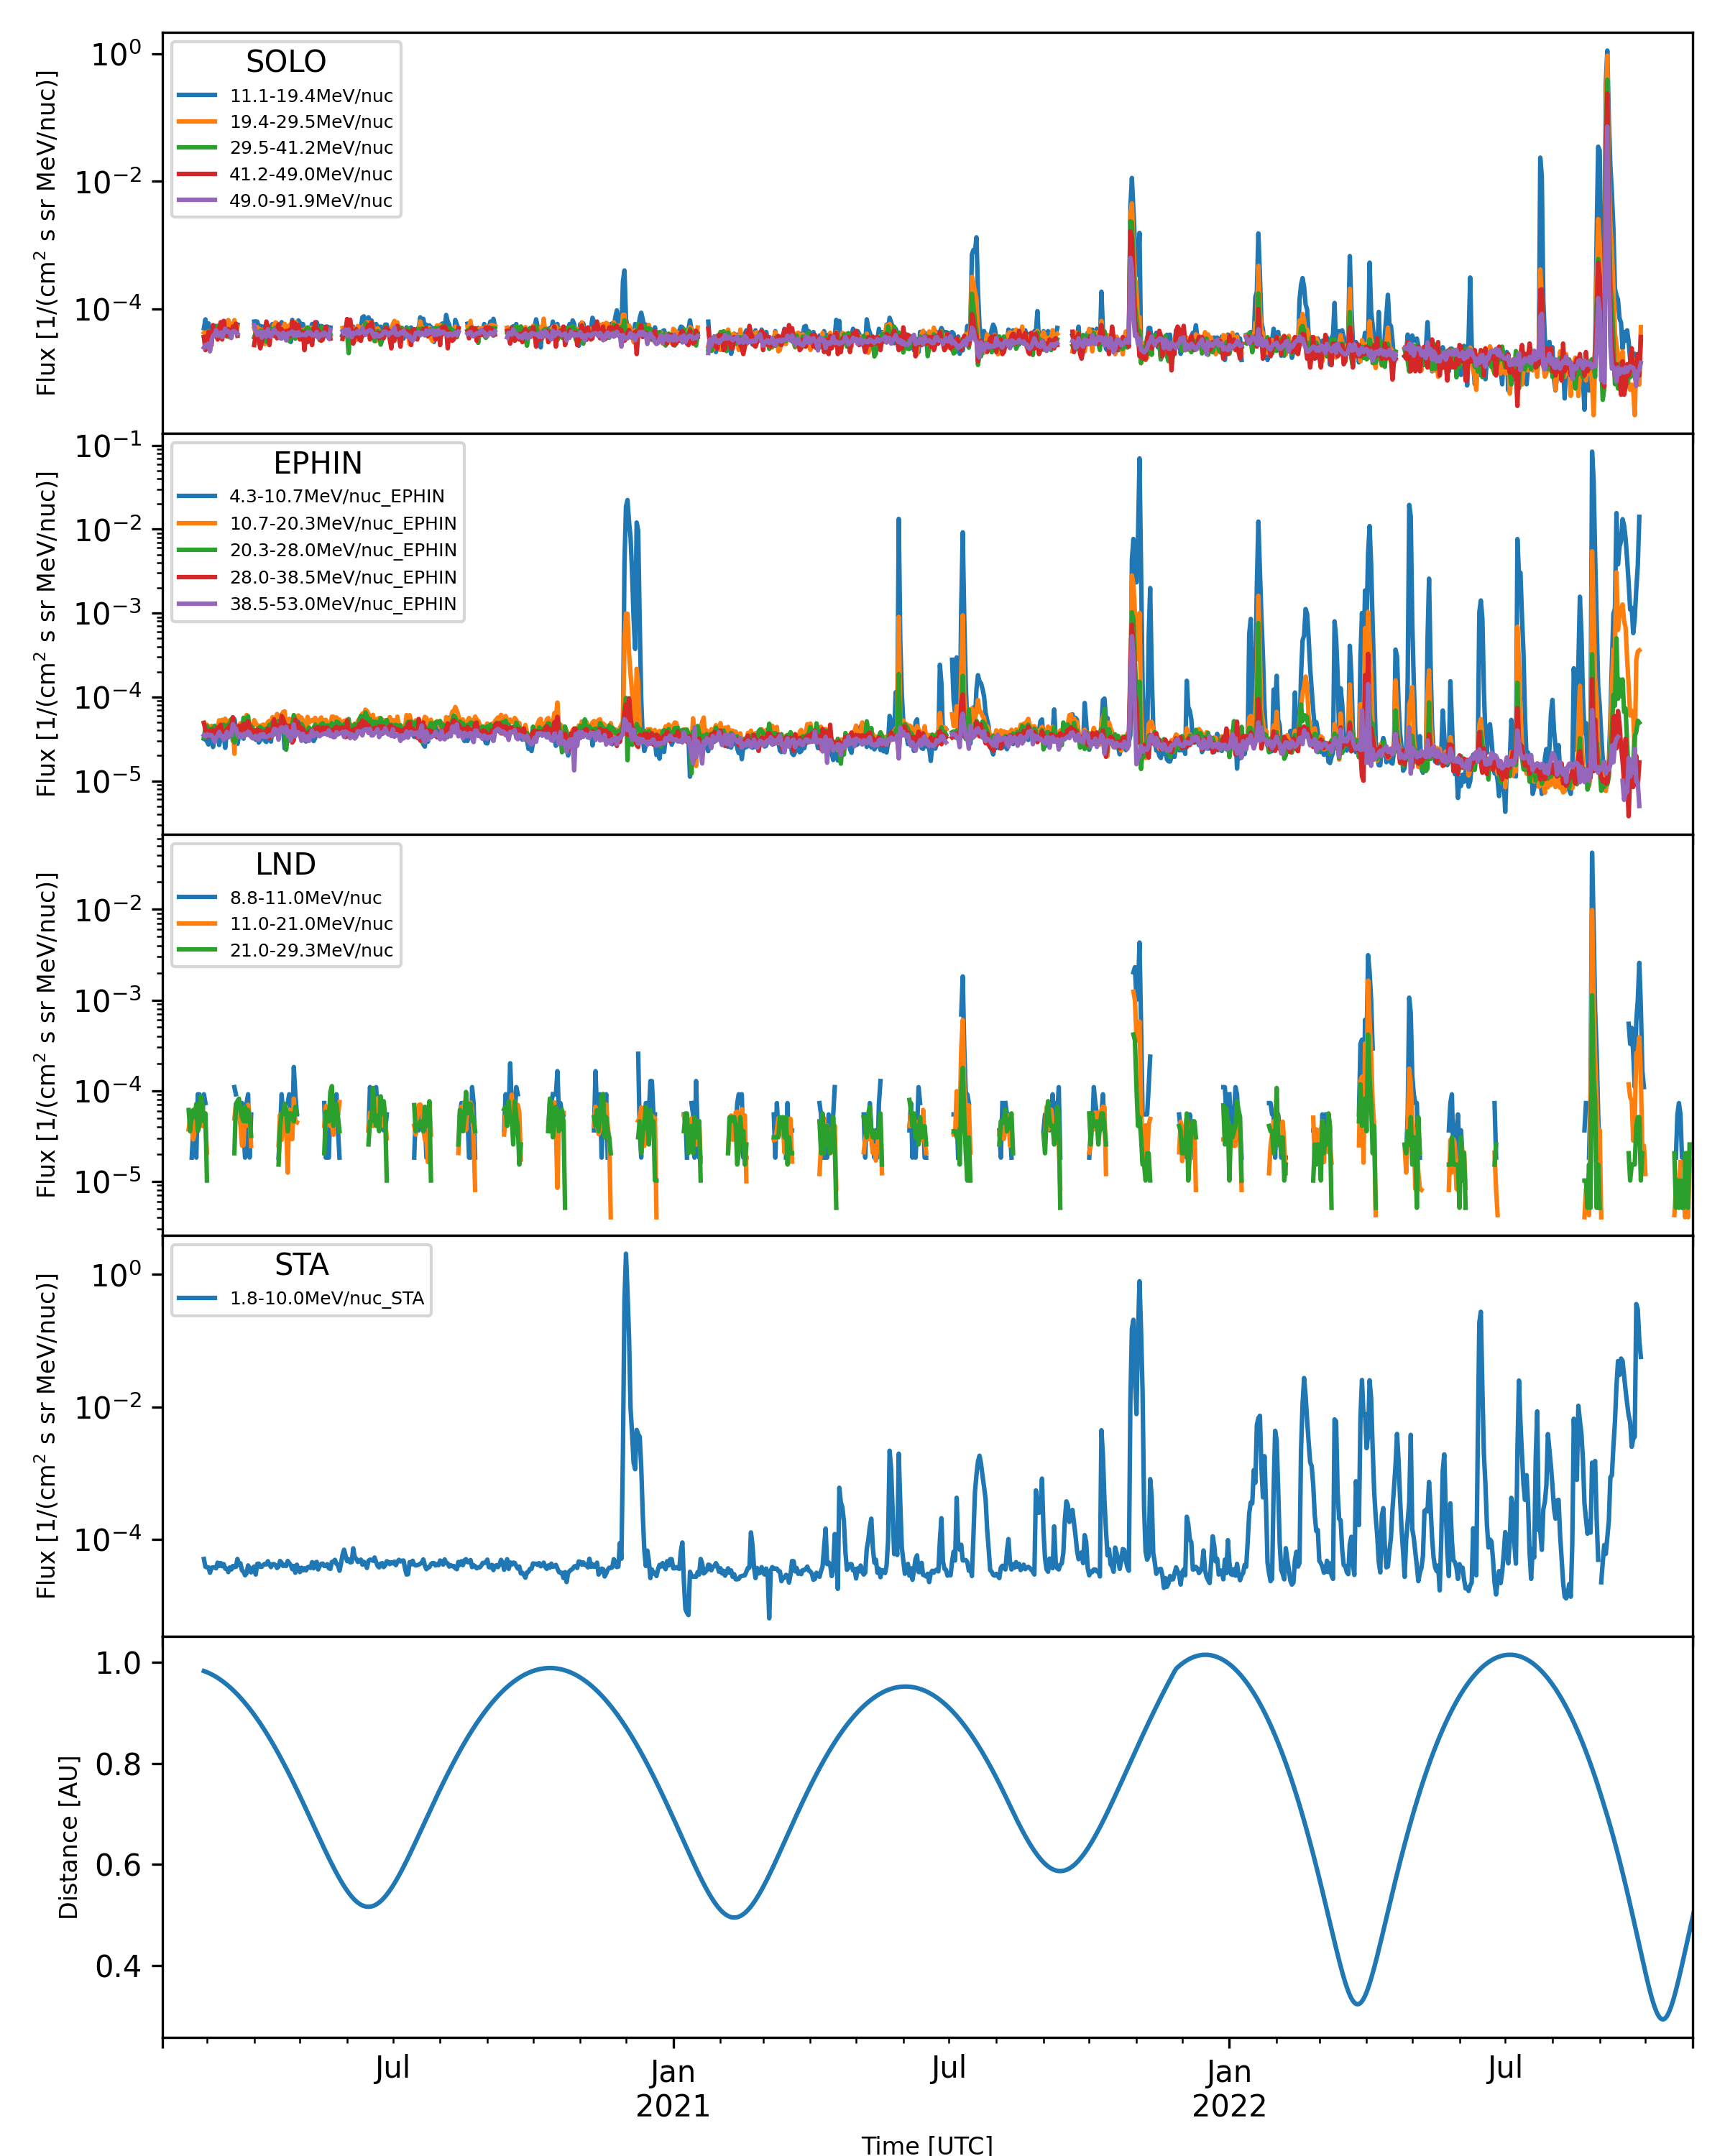
\includegraphics[width = 0.8\textwidth]{images/ACR/overview_Helium_4_instrument.png}
    \caption{The daily averaged Helium flux measured by (from top to the bottom) SOLO/HET, SOHO/EPHIN, Chang'E-4/LND, and STA/LET between Feb 2020 and October 2022. The bottom plot show the radial distance of SOLO during the corresponding periods.
    %The red dashed lines indicate the SEP events that we determined by eye.
    \TODO{reminder: you should better re-load the SOLO data, and check the isotropic between different direction, and resample data before further process like sum all direciton or somesome.}}
    \label{fig:overview}
\end{figure}


Based on the orbit information, we could easily determind the period, when \ac{SolO} located near 1 au. such a list of periods in the last two years is given in Tab.~\ref{tab:1AU_period}.

\begin{table}[]
    \centering
	\caption{The list of time perods when the solar radial distance of \ac{SolO} is between 0.95 and 1 AU}
	\label{tab:1AU_period}
    \begin{tabular}{|c|c|c|c|}
	periods & start time & end time & distance to Earth \\
	1	& 2020-09-14 & 2020-11-10	& 1 \\
	2	& 2021-05-27 & 2021-06-09	& 1 \\
	3	& 2021-11-21 & 2022-01-15	& 1 \\
	4	& 2022-06-05 & 2022-08-02	& 1 \\
    \end{tabular}
\end{table}


To further compare and cross calibrate the measurement between different instrument, we extracted the data when the SOLO is located between 0.95 and 1 au. These period are marked out by the shadow region in the \ref{fig:overview}. The corresponding spectra are given in Fig.\ref{fig:spec}. 
We could 
Spectra.

\begin{figure}
    \centering
    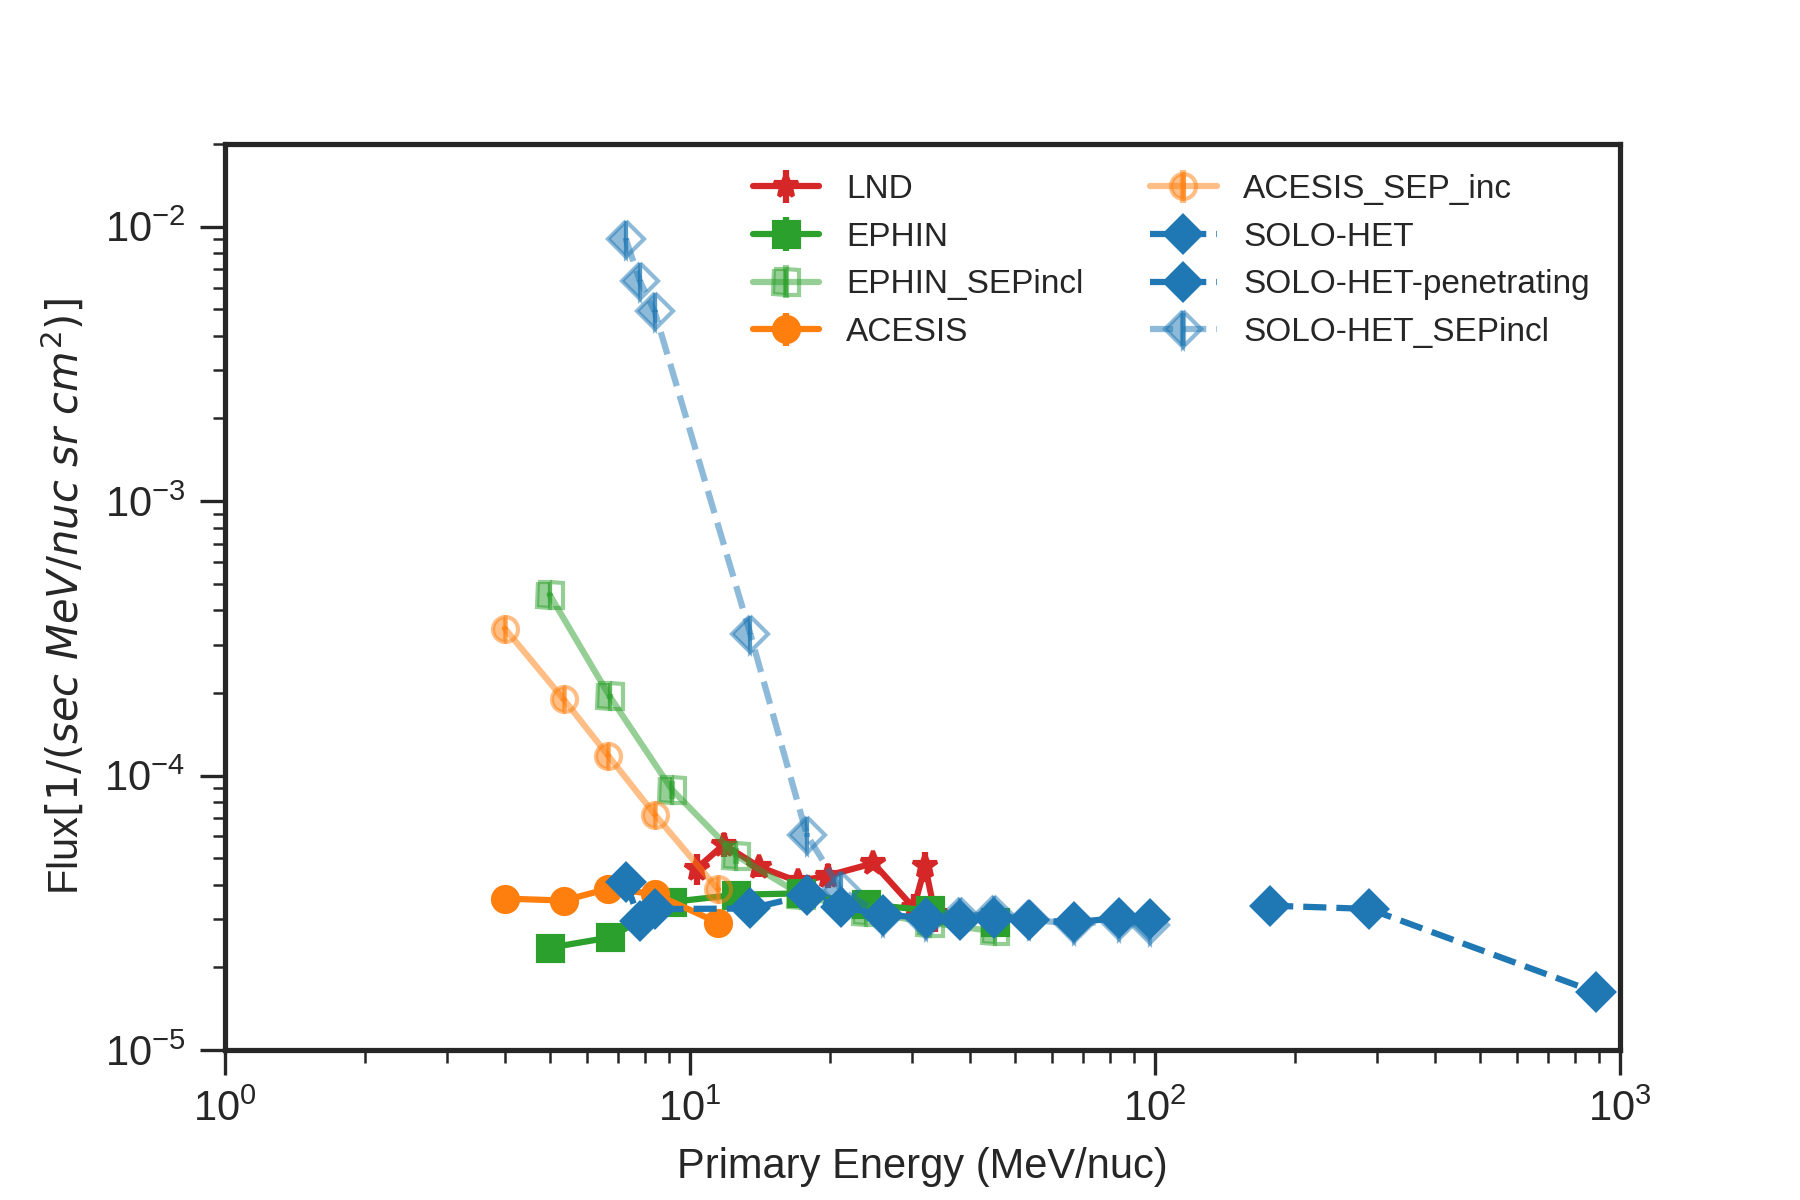
\includegraphics[width = 0.8\textwidth]{images/ACR/1AU_comparison_ACE_EPHIN_SOLO_SEPIncl_Helium.png}
    \caption{The helium-4 spectra of SOLO/HET, SOHO/EPHIN, ACE/SIS and Chang'4/LND when SOLO was between 0.95 and 1AU. The light colored data points are the spectra including SEPs and the others represent the quite time spectra.}
\end{figure}

Considering the energy coverage of different L1 instruments we utitlized before and for the convinence of the comparison with SOLO, in the following chapter, we only consider the SOHO/EPHIN which could cover the energy between 10 - 50 MeV/nuc as the base line of SOLO.

\subsection{}

\subsection{Generate the SEP list and remove the SEP events}

\subsection{}

\section{Results and summary}







%\input{chapters/pub04_xu2022}
